% Unofficial UChicago CS Poster Template
% v1.1.0 released September 8, 2022
% https://github.com/k4rtik/uchicago-poster
% a fork of https://github.com/anishathalye/gemini

\documentclass[final]{beamer}

% ====================
% Packages
% ====================

\usepackage[T1]{fontenc}
\usepackage{lmodern}
\usepackage[size=custom,width=120,height=72,scale=1.0]{beamerposter}
% \usepackage[size=custom,width=90,height=60,scale=1.0]{beamerposter}
\usetheme{gemini}
\usecolortheme{uchicago}
\usepackage{graphicx}
\usepackage{booktabs}
\usepackage{bm}
\usepackage[ruled]{algorithm2e}
%\usepackage{enumitem}
\usepackage{doi}
\usepackage[numbers]{natbib}
\usepackage[patch=none]{microtype}
\usepackage{arydshln}
\usepackage{tikz}
\usepackage{pgfplots}
\pgfplotsset{compat=1.18}
\usepackage{anyfontsize}
\usepackage{subcaption}
\usepackage{wrapfig}
\usepackage{outlines}
\usetikzlibrary{arrows,shapes}

\pdfstringdefDisableCommands{%
\def\translate#1{#1}%
}

% ====================
% Lengths
% ====================

% If you have N columns, choose \sepwidth and \colwidth such that
% (N+1)*\sepwidth + N*\colwidth = \paperwidth
\newlength{\sepwidth}
\newlength{\colwidth}
\setlength{\sepwidth}{0.015\paperwidth}
\setlength{\colwidth}{0.31\paperwidth}

\newcommand{\separatorcolumn}{\begin{column}{\sepwidth}\end{column}}

% ====================
% Title
% ====================

\title{Exploring Robustness of Stanford's DeepSolar Model to Distribution Shifts}

\author{Kerrie Wu (kerriewu@stanford.edu) \and Julian Cooper (jelc@stanford.edu) \and Andrea van den Haak (vandenhaak@stanford.edu)}


% ====================
% Footer (optional)
% ====================

%\footercontent{
%  \href{https://www.example.com}{https://www.example.com} \hfill
%  CS229 Poster session, Stanford University --- XYZ-1234 \hfill
%  \href{mailto:alyssa.p.hacker@example.com}{alyssa.p.hacker@example.com}}
% (can be left out to remove footer)

% ====================
% Logo (optional)
% ====================

% use this to include logos on the left and/or right side of the header:
% \logoright{\includegraphics[height=7cm]{logo1.pdf}}


% ====================
% Body
% ====================

\begin{document}
\addtobeamertemplate{headline}{}
{
    \begin{tikzpicture}[remember picture,overlay]
     % \node [anchor=north west, inner sep=3cm] at ([xshift=0.0cm,yshift=1.0cm]current page.north west)
      %{\includegraphics[height=5.0cm]{logos/uc-logo-white.eps}}; % also try shield-white.eps
      \node [anchor=north east, inner sep=2.3cm] at ([xshift=0.0cm,yshift=2.5cm]current page.north east)
      {
\includegraphics[height=7.5cm]{stanford.png}};
    \end{tikzpicture}
}


\begin{frame}[t]
\vfill

% \begin{frame}[t]
\begin{columns}[t]
\separatorcolumn

\begin{column}{\colwidth}

\begin{block}{\large Introduction \& Background}
  % \centering
\begin{itemize}
    \item \textbf{In many countries, the rollout of rooftop solar has been ad hoc and largely untracked}. Being able to estimate rooftop solar adoption allows utilities to predict power output reasonably well and make the adjustments to grid management and investment.[2] \\[20pt]
    
    \item In December 2018, Stanford's Deepsolar team produced an aerial imagery dataset and model which together largely solved this challenge for the United States [1]. However, even in its current form, the \textbf{Deepsolar model is not robust to "distribution shifts"}. \\[20pt]
    
    \item In January 2023, Kasmi et al. published a new dataset for residential areas in France. As feared, Stanford's Deepsolar performed poorly: \textbf{classification F1 score fell from 0.91 to 0.24} and \textbf{segmentation IOU fell from 0.51 to 0.06}.

\end{itemize}

\end{block}

\begin{block}{\large Problem Statement}
  % \centering

Our goal is to adapt DeepSolar's model to new domains and improve its overall robustness to domain shifts while using minimal domain-specific labeled data. \\[20pt]

We explore two data-efficient techniques for improving the DeepSolar model's performance on the French dataset: \textbf{regularized fine-tuning} and \textbf{interpolation-based data augmentation}. 

\end{block}

\begin{block}{\large Datasets \& Pre-Processing}
  % \centering
\begin{minipage}[t]{0.45\linewidth}
    
\textbf{United States} (Deepsolar, 2018) [1]
Heavily skewed, larger dataset covering all parts of the contiguous United States.
\begin{itemize}
  \item 46,090 images with solar panels, 366,467 images without
  \item 3 x 320 x 320 input image size
  \item Industrial and residential regions
  % \item Classification labels and ground truth segmentation masks
\end{itemize}

\begin{figure}
\centering
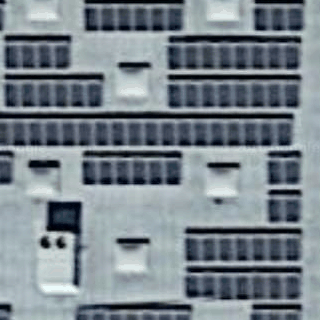
\includegraphics[width=11.5cm]{img_usa.png}
\end{figure}

\end{minipage}%
\hfill%\vline\hfill
\begin{adjustbox}
\begin{minipage}[t]{0.45\linewidth}

\textbf{France} (Kasmi et al., 2023) [2]
Class balanced, smaller dataset covering primarily residential areas of France. 
\begin{itemize}
  \item 13,303 images with solar panels, \\
  15504 images without
  \item 3 x 400 x 400 input image size
  \item Residential regions only
  % \item Classification labels and ground truth segmentation masks
\begin{figure}
\centering
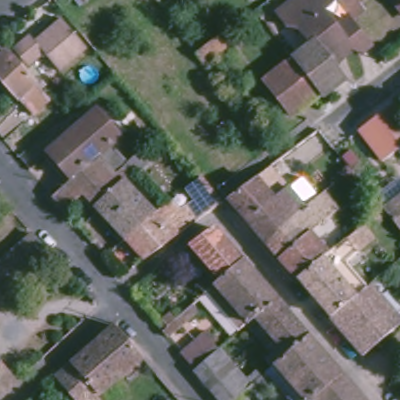
\includegraphics[width=12cm]{img_french.png}
\end{figure}
\end{itemize}

\end{minipage}
\end{adjustbox}
\vspace{48pt}
\linebreak
\textbf{Image pre-processing pipeline}: Significant work was required to wrangle the French dataset into a state usable with selected components of the existing Deepsolar training pipeline.
\begin{itemize}
  \item Data augmentation transforms including random 90-degree rotations and horizontal flips
  \item Resize images to 299 $\times$ 299 to match the Inception3 model's input API 
  \item Normalize mean and standard deviation of each channel
  \item Split dataset into test (5000 images), validation (1000 images), and training (remainder)
  \item Create class-balanced finetuning sets with 100, 500, 1000, and 5000 images per class
\end{itemize}

\end{block}
\end{column}

\separatorcolumn

\begin{column}{\colwidth}

\begin{block}{Method 1: Regularized Finetuning}
% Without regularization, finetuning routines suffer from overfitting.
\textbf{L2 regularization}: Use the Adam optimizer and tune weight decay and learning rate. Weight decay constant guarantees we do not take too large steps away from pretrained weights. \\[20pt]
    
\textbf{Adversarial regularization}: When the input $x$ is perturbed by a small amount, the output should not change much. To achieve this, Jiang et al. optimize loss $\mathcal{F}(\theta)$ using: $\min_{\theta} \mathcal{F}(\theta) = \mathcal{L}(\theta) + \lambda_{s}\mathcal{R}_{s}(\theta)$, where $\mathcal{R}_{s}(\theta) & = \frac{1}{n} \sum_{i=1}^{n} \max_{\lVert \Tilde{x_{i}} - x_{i} \rVert_{p \leq \epsilon}} l_{s}\left(f(\Tilde{x_{i}}; \theta), f(x_{i}; \theta)\right)$.
% \begin{align*}
% \mathcal{L}(\theta) & = \frac{1}{n} \sum_{i=1}^{n} l(f(x_{i};\theta), y_{i})  \\
% \mathcal{R}_{s}(\theta) & = \frac{1}{n} \sum_{i=1}^{n} \max_{\lVert \Tilde{x_{i}} - x_{i} \rVert_{p \leq \epsilon}} l_{s}\left(f(\Tilde{x_{i}}; \theta), f(x_{i}; \theta)\right) \\
% \end{align*} 

\end{block}

\begin{block}{Method 2: LISA Data Augmentation}

LISA [3] is a data augmentation method that uses \textbf{linear interpolation between training examples} to improve model robustness to distribution shifts.

\begin{figure}
\centering
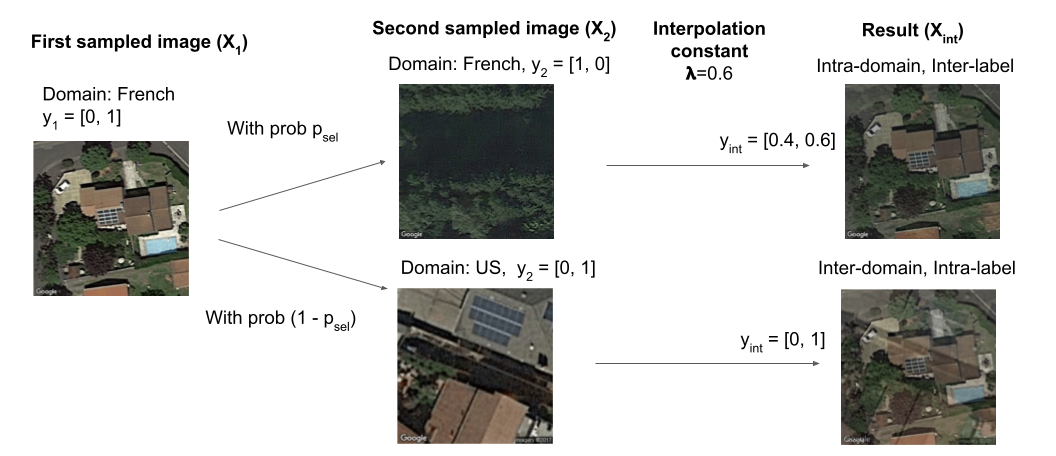
\includegraphics[width=0.9\linewidth]{lisa_viz_poster.png}  
\end{figure}

\begin{enumerate}
\item Select a training example and label $X_1 , y_1$ from the French finetuning dataset
\item Sample a $\lambda$ value in the range [0, 1] from a $Beta(2,2)$ distribution
\item Select a second example and label $X_2, y_2$ for either inter-label or inter-domain interpolation
\item Resize both $X_1$ and $X_2$ to the input size for the model
\item Construct $X_{int} = \lambda X_1 + (1 - \lambda)X_2$, and  $y_{int} = \lambda y_1 + (1 - \lambda)y_2$
\end{enumerate}

\end{block}

\begin{block}{Experimental Results}
Summary of our key experimental results, including classification and segmentation performance metrics for our finetuned model variants on the test French dataset. \vspace{-20pt}
\begin{table}
\begin{center}
\begin{tabular}{lcccccccc}
&  & \multicolumn{1}{l}{} 
   & \multicolumn{4}{c}{\textit{Classification}}                       
   & \multicolumn{2}{c}{\textit{Segmentation}} \\ 
\hline
Model & \begin{tabular}{@{}c@{}}Eval\\Dataset\end{tabular} & \begin{tabular}{@{}c@{}}No.\\rows\end{tabular} & \multicolumn{1}{c}{Accuracy} & \multicolumn{1}{c}{F1 Score} & \multicolumn{1}{c}{Precision}  & \multicolumn{1}{c}{Recall} & \begin{tabular}{@{}c@{}}Area \\ Error\end{tabular} & \multicolumn{1}{c}{IOU} \\ \hline
Deepsolar Baseline & USA & n/a & 0.99 & 0.91 & 0.95 & 0.86 & -0.08  & 0.51 \\
Deepsolar Baseline & FR & n/a & 0.57 & 0.24 & 0.96 & 0.14 & -0.73 & 0.06 \\ 
\hline
Regularized Finetuning & FR & 100 & 0.87 & 0.87 & 0.86 & 0.89 & 0.10 & 0.23 \\
Regularized Finetuning & FR & 500 & 0.94 & 0.94 & 0.97 & 0.91 & -0.24 & 0.48 \\
Regularized Finetuning & FR & 1000 & 0.97 & 0.96 & 0.96 & 0.97 & 0.10 & 0.52 \\
Regularized Finetuning & FR & 5000 & 0.98 & 0.98 & 0.97 & 0.99 & -0.02 & 0.54 \\ 
\hline
LISA Data Augmentation &  FR  & 100 &  0.87 & 0.88 & 0.81 & 0.98 & 0.02 & 0.31 \\
LISA Data Augmentation &  FR  & 500 &  0.95 & 0.95 & 0.95 & 0.96 & 0.07 & 0.40 \\
LISA Data Augmentation &  FR  & 1000 &  0.97 & 0.97 & 0.96 & 0.98 & -0.04 & 0.10 \\
LISA Data Augmentation &  FR  & 5000 &  0.97 & 0.97 & 0.96 & 0.98 & -0.04 & 0.38 \\
\hline
\end{tabular}
\end{center}
%     \caption{Summary of experimental results showing performance of (1) the Deepsolar Baseline model (pretrained) on the original US dataset compared to results with the same model on the French dataset; and (2) the Regularized Fine-tuning and LISA Data Augmentation model variants trained on varying quantities of labeled data from the target (French) datatset. 
%     % For each, we consider accuracy, precision and recall for the classification component, as well as area error (predicted area - true area) / true area) and intersection over union (IOU) for segmentation. We also compare US dataset results to those of the original Deepsolar US model but using Facebook's Segment Anything Model for segmentation. 
%     Accuracy, Precision and Recall are all based on the image classification performance of the model. Area error measures the relative difference between the predicted solar PV area and the true solar PV area as measured by the true segmentation masks. IOU stands for intersection over union which is our primary measure of correctness for the segmentation task.}
% \end{center}
\label{table:results}
\end{table}
\end{block}
% \begin{block}{Model and Finetuning Procedure}
% \textbf{The DeepSolar model consists of an Inception3 CNN classification backbone and 2-convolutional-layer auxiliary segmentation branch that stems from an intermediate classification branch layer.} 

% For each method, we use the Adam optimizer and tune each step separately using either grid search or Bayesian hyperparameter optimization. 
% \begin{enumerate}
% \item \textbf{Finetune the entire classification branch}, initialized from the pretrained DeepSolar baseline model. \textbf{Freeze the classification branch parameters}. 
% \item \textbf{Finetune the first convolutional layer of the segmentation branch}, initialized from the original DeepSolar model parameters, using a classification objective.  \textbf{Freeze this layer of the segmentation branch.}
% \item \textbf{Repeat Step 2 for the second convolutional layer of the segmentation branch.}
% \end{enumerate}
% \end{block}

\end{column}

\separatorcolumn

\begin{column}{\colwidth}

\begin{block}{Discussion \& Error Analysis}
\begin{minipage}[t]{0.45\linewidth}
\begin{itemize}
    \item \textbf{Image misclassification}: The most significant difference between the original Deepsolar baseline and our finetuned model variants (Fig, row 2). The baseline model achieved precision of 0.96 but recall of only 0.14. This means it was confident in the images it did select but misclassified many images that did in fact have solar panels. For those images, it predicted an empty segmentation! \\[20pt]
    
    \item \textbf{Object confusion}: Initially, a large source of error was object confusion (Fig, row 4). As we add more data from the French dataset, which is more heavily weighted towards residential settings, our models improved at correctly identifying objects. For example, in row 5 we no longer confuse a swimming pool for a solar panel. \\[20pt]

    \item \textbf{Diffuse prediction error}: Our last common source of error was placing high probabilities on area surrounding the solar panel (often rooftop). To address this, we tuned our CAM segmentation threshold (how confident we need to be for a pixel to be considered 1 vs 0) as an additional hyperparameter. This improved total area error but not IOU since our model will often put comparable weight on solar panels and other roof elements!
    
\end{itemize}

\end{minipage}
\hfill %\vline\hfill
\begin{minipage}[t]{0.5\linewidth}
\begin{figure}
\centering
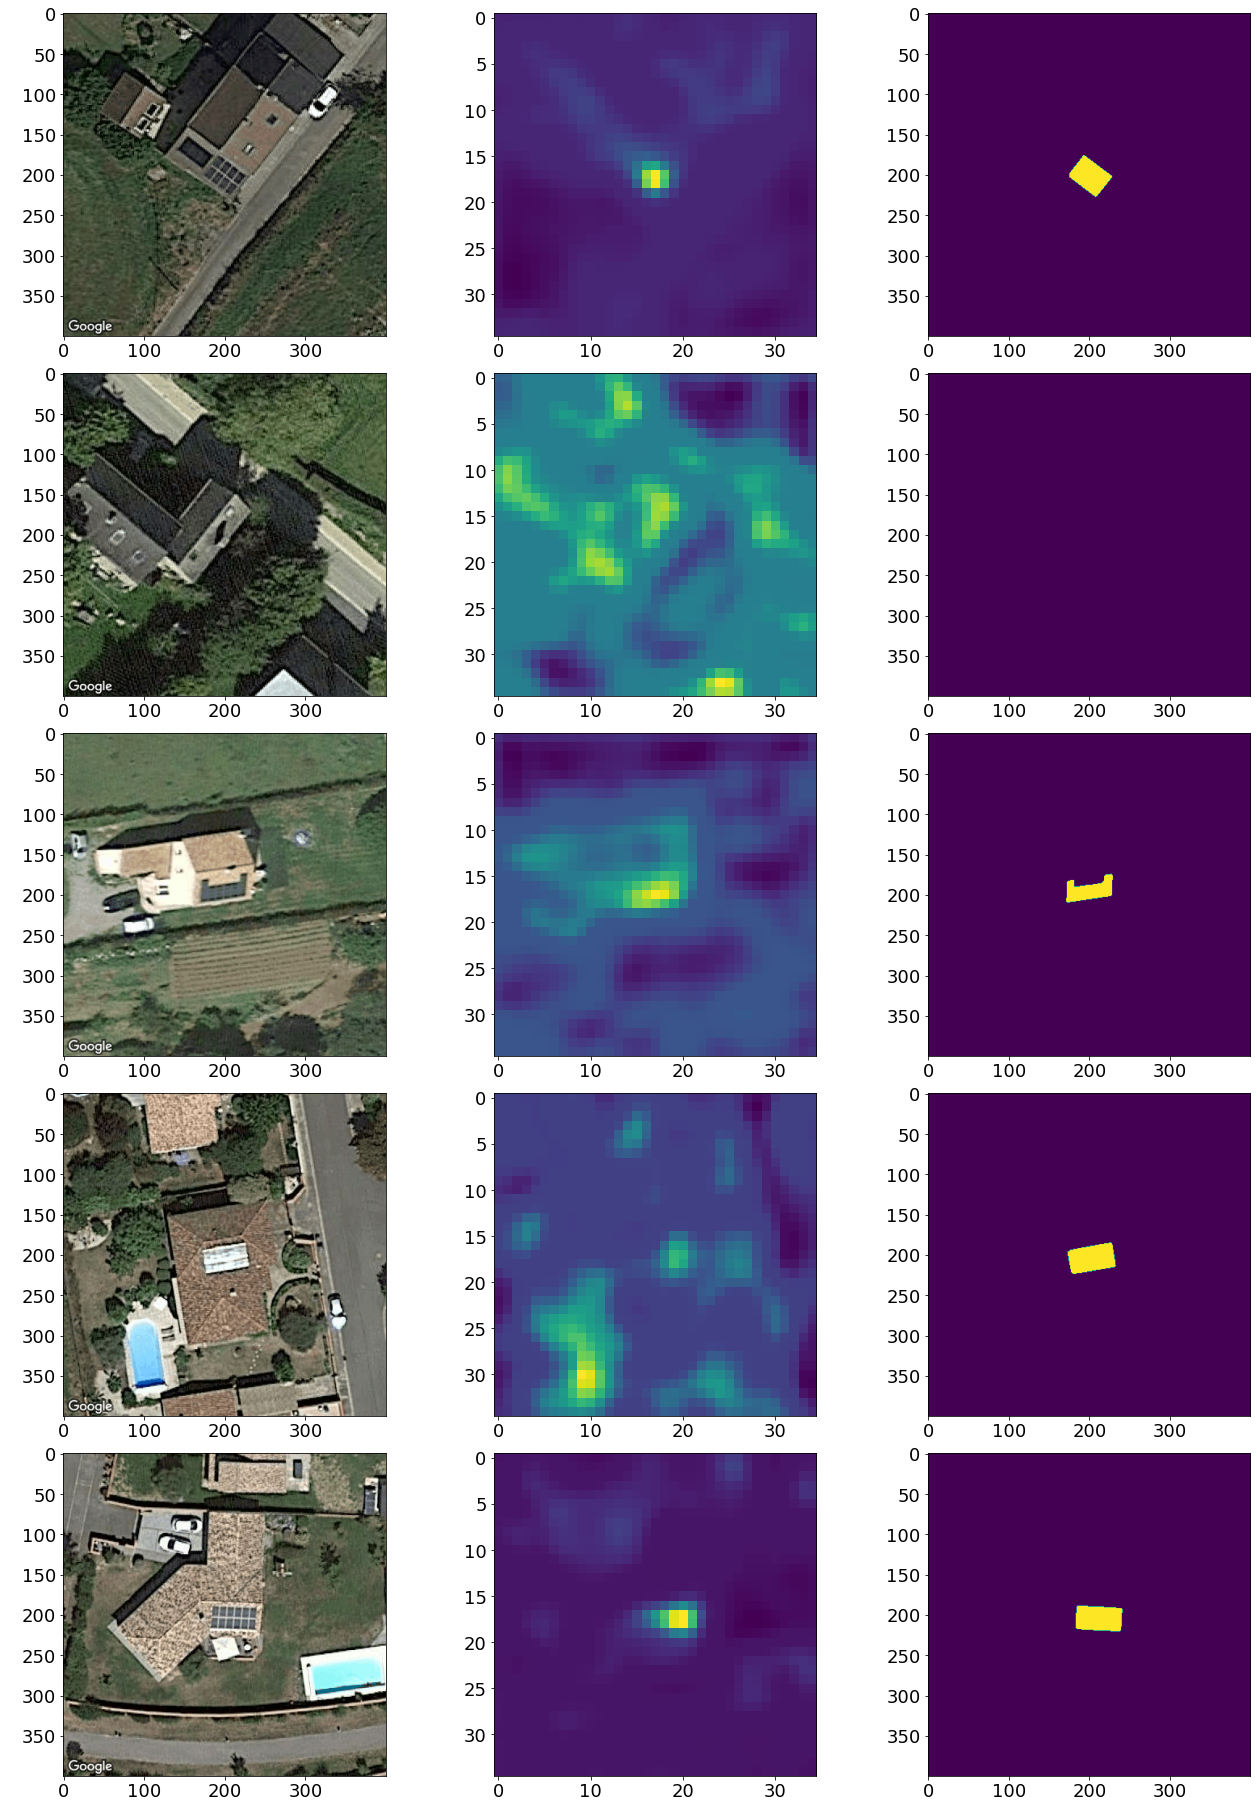
\includegraphics[width=\linewidth]{good_bad_examples.png}
\end{figure}
Example input images (left), CAM outputs (middle), and true segmentation masks (right). Rows: (1) good example of simple segmentation; (2) bad example of model misclassification; (3) bad example of overly diffuse prediction; (4) bad example of confusing objects; (5) good example of handling similar objects. 

\end{minipage}
\end{block}

\begin{block}{Conclusion and Future Work}
% \begin{minipage}[t]{0.5\linewidth}
% \textbf{Main takeaways}:
\begin{itemize}
    \item We are able to achieve \textbf{comparable classification and segmentation performance on a new domain} by finetuning the DeepSolar on only 500 per-class labeled  samples from the target data distribution using either L2 regularization or LISA. \\[20pt]
    
    \item \textbf{However, neither method improved model robustness} to distribution shifts in general. The finetuned models performed well on the French dataset, but poorly on the US dataset. \\[20pt]
    
    \item Future work should include expand this investigation to include additional known distribution shift techniques such as Domain Adaptation and General Adversarial Networks.

\end{itemize}
% \end{minipage}
% \hfill\vline\hfill
% \begin{minipage}[t]{0.4\linewidth}
% \textbf{Potential future directions include}: 
% \begin{itemize}
%     \item Try finetuning with other data augmentation techniques, including using GANs
%     \item Investigate if choosing a lower $p_{sel}$ value when finetuning with LISA could improve model robustness to distribution shifts.

% \end{itemize}
% \end{minipage}
\end{block}



\begin{block}{Acknowledgements}
We would like to thank Zhecheng Wang for providing us with initial guidance on directions for this project, introducing us to the DeepSolar Github repository, and providing us with the DeepSolar US dataset. 
\end{block}

  %   \begin{alertblock}{\small Future Work}

  %   \begin{itemize}
  %   \item Expand this investigation to include additional known distribution shift techniques such as Domain Adaptation and General Adversarial Networks (GANs)
  %   \item Investigate if choosing a lower $p_{sel}$ value when finetuning with LISA could improve model robustness to distribution shifts
    
  %   \end{itemize}
  % \end{alertblock}

\end{column}

\separatorcolumn
\end{columns}
\begin{alertblock}
\footnotesize
\begin{enumerate}
\item Jiafan Yu, Zhecheng Wang, Arun Majumdar, and Ram Rajagopal. Deepsolar: A machine learning framework to efficiently construct a solar deployment database in the united states. Joule, 2(12):2605–2617, 2018.  \\
\item Gabriel Kasmi, Yves-Marie Saint-Drenan, David Trebosc, Raphaël Jolivet, Jonathan Leloux, Babacar Sarr, and Laurent Dubus. A crowdsourced dataset of aerial images with annotated solar photovoltaic arrays and installation metadata. Scientific Data, 10(1):59, Jan 2023.\\
\item Huaxiu Yao, Yu Wang, Sai Li, Linjun Zhang, Weixin Liang, James Zou, and Chelsea Finn. Improving outof-distribution robustness via selective augmentation, 2022
\end{enumerate}
\end{alertblock}
% \begin{block}

%     % \nocite{*}
%     \footnotesize{\bibliographystyle{plainnat}\bibliography{poster}}

% \end{block}

\end{frame}

\end{document}
